%!TeX root = Chapter_IceTheory
\documentclass[../../CompleteThesis/Complete_1stDraft.tex]{subfiles}
\begin{document}
	
	\section[Water Isotopes][Water Isotopes]{Water Isotopes and $\delta$-notation}
	\label{Sec:Ice_WaterIsotopes}
	A corner stone in ice core analysis, which helps lay the basis for paleo climate research, is through measurements of the isotopic composition of the water - or that of the encapsulated air in bubbles - which makes up the ice cores. Water isotopes are sensitive to temperature changes and can thus be used as a proxy for paleo temperature along with being used as dating parameters, since the annual cycles often are detectable in water isotope data.
	
	\begin{figure}[h]
		\centering
		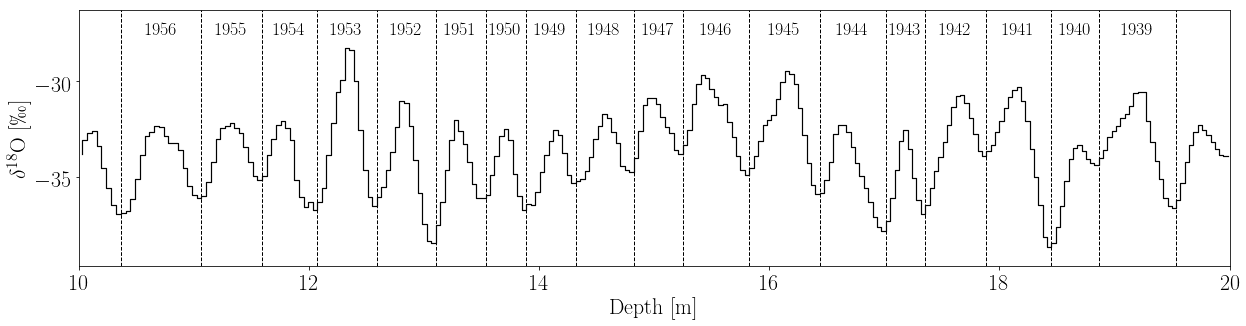
\includegraphics[width=\textwidth]{Crete_10m_dated.png}
		\caption{Ten meters of the top of Cretê ice core, with identification and dating of 19 annual layers.}
		\label{Fig:ICE_Crete_10m_dated}
	\end{figure}
	
	\subsection[$\delta$ notation]{$\delta$ notation and water isotopes}
	\label{Subsec:Ice_WaterIsotopes_deltaNotation}
	
	\todo{ICE-ISO: Implement illustration of fractionation and deposition}
	Water isotopic ratios, i.e. the ratio of the minority isotope, ${\text{H}_2^{18}\text{O}}$ or ${\text{H}_2^{17}\text{O}}$($^2\text{H}_2\text{O}$), compared to the majority isotope, ${\text{H}_2^{16}\text{O}}$ ($^1\text{H}_2\text{O}$), are used to report the quantities of isotopes in a sample relative to the ratio of a given reference water sample. This is commonly expressed in the $\delta$-notation as:
	\begin{equation}
		\delta^i = \frac{^iR_{sample}}{^iR_{reference}} - 1		
	\end{equation}
	where $^{18}R = \frac{n_{^{18}\text{O}}}{n_{^{16}\text{O}}}$, $^{2}R = \frac{n_{^{2}\text{H}}}{n_{^{1}\text{H}}}$  and $^{17}R = \frac{n_{^{17}\text{O}}}{n_{^{16}\text{O}}}$. Here n is the abundance of the given isotope.\\
	Besides the isotopic quantities $\delta^{17}\text{O}$, $\delta^{18}\text{O}$ and $\delta^2\text{H} = \delta\text{D}$, both deuterium excess and $\Delta^{17}\text{O}$, known as $^{17}\text{O}$ excess, can be of interest. Deuterium excess is usually used as a measure of the kinetic fractionation processes, taking place in the water vapor formation of polar precipitation, giving an indicator of the conditions during precipitation formation, and thus giving a pointer to the source of the water vapor.
	Like deuterium excess $^{17}\text{O}$ is sensitive to kinetic fractionation, but much less sensitive to equilibrium fractionation than both $\delta$D and $\delta^{18}$O. Along with being nearly insensitive to temperature(REFERENCES), these robustness factors leads to $^{17}$O being usable as an independent parameter to be used to reveal the ways of the complicated mixing effects of fractionation due to evaporation, transportation, formation and deposition.
	
	
	\section[Diffusion and Densification][Diffusion and Densification]{Diffusion and Densification}
	\label{Sec:Ice_DiffusionAndDensification}
	Throughout the firn column the important processes of diffusion and densification takes places. Both processes need to be well understood and examined when analyzing ice core data, as diffusion and densification play a large role in thinning of annual layers due to compression of snow to ice and in washing out the measured signals through diffusion in the firn.
	\todo{ICE-ISO: Write about isotopes and temperature relations}
	\subsection[Densification][Densification]{Densification}
	\label{Subsec:Ice_DiffusionAndDensification_Densification}
	Densification is the process of compression of snow to ice. It plays an important role in the annual layer thickness in the data as snow will be compressed to a smaller volume under pressure from the firn column above until it reaches a solid ice state with a, almost, constant density. \\
	Commonly three stages of densification are described in the firn column. The first stage is between the initial precipitated snow density and the 'critical density' at $0.55 \frac{\text{Mg}}{\text{m}^3}$, the second stage is between critical density and the close-off density at $0.82-0.84 \frac{\text{Mg}}{\text{m}^3}$, and the third stage is from close-off and all the way through the ice.\\
	At the first stage the densification is mostly due to grain settling and packing and the densification rate is very rapid. At the second stage, the snow is close to isolating air bubbles. At the third stage, the dominating densification taking place is by the compression of air bubbles.\\
	For these three stages it is of interest to develop a depth-density profile, which is dependent on snow accumulation rate and temperature. The focus is on developing an empirical model for the first and second stages of densification, as they are the most dramatic sections of the firn column considering densification and diffusion.\\
	A number of different densification models have been developed(REFERENCES), and in this thesis will be presented the ones used for the analysis.
	\subsubsection{Herron Langway Empirical Model}
	\label{Subsubsec:Ice_DiffusionAndDensification_Densification_HL}
	Sorge's law(REFERENCES) assumes that the relation between snow density $\rho$ and depth $h$ is invariant with time, given a constant snow accumulation and temperature. Furthermore, annual layer thinning by plastic flow is ignored.\\
	Densification of firn, which can be described as the proportional change in air space, is linearly related to change in stress due to the weight of the overlying snow(REFERENCES):
	\begin{equation}
		\frac{d\rho}{\rho_i - \rho} = \text{const.} \, \rho \, dh
		\label{Eq:Dens_Prop_Stress}
	\end{equation}
	By integration, this implies a linear relation between $\ln\left[\frac{\rho}{\rho_i - \rho}\right]$ and $h$.\\
	When considering real data, analysis shows that $\ln\left[\frac{\rho}{\rho_i - \rho}\right]$ vs $h$. plots have two linear segments(EXAMPLE), corresponding to the first and second stages of densification, with separation of segments at $\rho = 0.55$ and $\rho = 0.8$. These segments on the plots will yield two different slopes with slope constants:
	\begin{subequations}
		\begin{center}
			
			\begin{tabularx}{\textwidth}{Xp{2cm}X}
				\begin{equation}
					C = \frac{d\ln\left[\frac{\rho}{\rho_i - \rho}\right]}{dh}, \rho < 0.55
					\label{Eq:Dens_Const_1}
				\end{equation}
				&&
				\begin{equation}
					C' = \frac{d\ln\left[\frac{\rho}{\rho_i - \rho}\right]}{dh}, 0.55 < \rho < 0.8
					\label{Eq:Dens_Const_2}
				\end{equation}
			\end{tabularx}
		\end{center}
	\end{subequations}
	To find the densification rate, $\frac{d\rho}{dt}$, substitute $\frac{dh}{dt} = \frac{A}{\rho} \rightarrow dt = \frac{\rho}{A} dh$ and use the differentiation $\frac{\partial}{\partial t}\left[\ln\left[\frac{x(t)}{k - x(t)}\right]\right] = \frac{k \frac{dx}{dt}}{(k - x(t))x(t)}$
	\begin{align*}
		C & = \frac{\rho}{A}\frac{d\ln\left[\frac{\rho}{\rho_i - \rho}\right]}{dt}\\
		& = \frac{\rho}{A} \frac{\rho_i}{\rho(\rho_i - \rho)}\frac{d\rho}{dt}\\
		& = \frac{1}{A}\frac{\rho_i}{\rho_i - \rho}\frac{d\rho}{dt}
	\end{align*}
	leading to 
	\begin{subequations}
		\begin{equation}
			\frac{d\rho}{dt} = \frac{C A}{\rho_i}(\rho_i - \rho)
			\label{Eq:Dens_Rate_1}
		\end{equation}
		\begin{equation}
			\frac{d\rho}{dt} = \frac{C' A}{\rho_i}(\rho_i - \rho)
			\label{Eq:Dens_Rate_2}
		\end{equation}
	\end{subequations}
	To continue from here two assumptions are made. The first is that the temperature and the accumulation rate dependencies may be separated, and that they thereby have no inter-correlation. The second is that the rate equations may be written as:
	\begin{subequations}
		\begin{equation}
			\frac{d\rho}{dt} = k_0 A^a (\rho_i - \rho), \rho < 0.55
			\label{Eq:Dens_Rate_1_Arrh}
		\end{equation}
		\begin{equation}
			\frac{d\rho}{dt} = k_1 A^b (\rho_i - \rho), 0.55 < \rho < 0.8
			\label{Eq:Dens_Rate_2_Arrh}
		\end{equation}
	\end{subequations}
	where $k_0$ and $k_1$ are Arrhenius type rate constants which are only temperature dependent, and $a$ and $b$ are constants determining the significance of the accumulation rate and are dependent on the densification mechanisms.\\
	$a$ and $b$ may be determined by comparing slopes for densification at different sites of nearly equivalent conditions as:
	\begin{equation}
		a = \frac{\ln\left(\frac{C_1}{C_2}\right)}{\ln\left(\frac{A_1}{A_2}\right)} + 1
		\label{Eq:Determ_const_a}
	\end{equation}
	and equivalently for b, with $C_1'$ and $C_2'$.\\
	$k_0$ and $k_1$ can be estimated by observing values of k at different temperatures and plotting $\ln(k)$ versus temperature - a so-called Arrhenius plot(REFERENCES) - to find $A$ and $E_a$ in equations:
	\begin{equation}
		k = A e^{-\frac{E_a}{k_B T}} = A e^{-\frac{E_a}{RT}}
	\end{equation}
	\begin{equation*}
		\ln(k) = \ln(A) - \frac{E_a}{R}\frac{1}{T}
	\end{equation*}
	leading to values of $k_0$ and $k_1$ of:
	\begin{subequations}
		\begin{center}
			
			\begin{tabularx}{\textwidth}{Xp{2cm}X}
				\begin{equation}
					k_0 = 11 e^{-\frac{10160}{RT}}
					\label{Eq:k0}
				\end{equation}
				&&
				\begin{equation}
					k_1 = 575 e^{-\frac{21400}{RT}}
					\label{Eq:k1}
				\end{equation}
			\end{tabularx}
		\end{center}
	\end{subequations}
	\textbf{Depth-density and depth-age calculations}\\
	Assuming that temperature, annual accumulation rate and initial snow density are known, the following calculations can be made:
	\begin{itemize}
		\item Density at depth $h$, $\rho(h)$
		\item Depth at pore close-off, $\rho=0.55$
		\item Depth-age relationship from surface to pore close-off (stage 1 and 2).
	\end{itemize}
	\textbf{1. stage of densification:}
	Depth-density profile:
	\begin{equation}
		\rho(h) = \frac{\rho_i Z_0}{1 + Z_0}
	\end{equation}
	where $Z_0 = e^{\rho_i k_0 h + \ln\left[\frac{\rho_0}{\rho_i - \rho_0}\right]}$. In this segment, the depth-density is independent of accumulation rate. The critical density depth can be calculated as:
	\begin{equation}
		h_{0.55} = \frac{1}{\rho_i k_0}\left[\ln\left[\frac{0.55}{\rho_i - 0.55}\right] - \ln\left[\frac{\rho_0}{\rho_i - \rho_0}\right]\right]
	\end{equation}
	and the age at close-off depth as:
	\begin{equation}
		t_{0.55} = \frac{1}{k_0 A}\ln\left[\frac{\rho_i - \rho_0}{\rho_i - 0.55}\right]
	\end{equation}
	
	\todo{ICE-DENS: Figure out where this comes from.}
	\textbf{2. stage of densificaion:} The depth-density profile
	\begin{equation}
		\rho(h) = \frac{\rho_i Z_1}{1 + Z_1}
	\end{equation}
	where $Z_1 = e^{\rho_i k_1 (h - h_{0.55})\frac{1}{A^{0.5}} + \ln\left[\frac{0.55}{\rho_i - 0.55}\right]}$. The age of firn at a given density $\rho$:
	\begin{equation}
		t_{\rho} = \frac{1}{k_1 A^{0.5}}\ln\left[\frac{\rho_1 - 0.55}{\rho_1 - \rho}\right]
	\end{equation}
	An estimate of the mean annual accumulation rate can be made from the slope $C'$ and the mean annual temperature:
	\begin{equation}
		A = \left(\frac{\rho_i k_1}{C'}\right)^2
	\end{equation}
	
	
	\begin{figure}
		\centering
		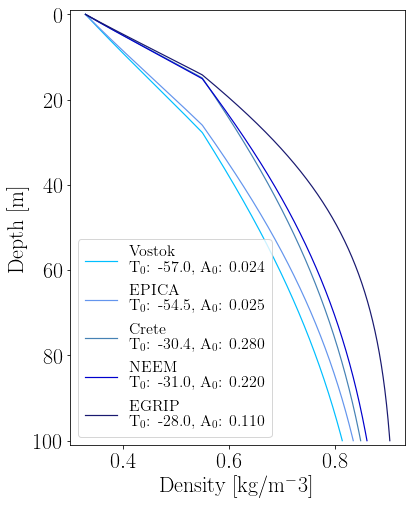
\includegraphics[width=0.6\textwidth]{DensProf_Examples.png}
		\caption{Density profile examples given five different initial conditions representing present day conditions at the five different ice core locations. Temperature, $T_0$, is in $^{\text{o}}$C and accumulation, $A_0$, is in meter of water equivalent per year.}
		\label{Fig:DensProf_Examples}
	\end{figure}
	
	
	
	\subsection[Diffusion]{Diffusion}
	\label{Subsec:Ice_DiffusionAndDensification_Diffusion}
	
	\subsubsection{In Firn}
	\label{Subsubsec:Ice_DiffusionAndDensification_Diffusion_Firn}
	Diffusion describes the attenuation of a given signal, e.g. a water isotopic signal, due to vapor phase diffusion in the porous firn column. This process takes place in the air pockets of the material from time of deposition to pore close-off. Commonly, firn is divided into three densification zones based on the dominant densification physics in the given zone \cite[Herron and Langway, 1980]{HerronLangway1980}, see section \ref{Sec:Densification}.
	To develop accurate knowledge of paleo climate and temperatures it is of great importance to understand this process, as a reconstruction of the part of the signal lost will reveal finer details in the signal and thus a more detailed knowledge of past times. 
	Diffusion can be described through Fick's $2^{\text{nd}}$ law, which describes the change in concentration of a substance with time, due to diffusion:
	\begin{equation}
		\frac{\partial \phi}{\partial t} = D(t) \frac{\partial^2 \phi}{\partial z^2} - \dot{\epsilon}_z(t) z \frac{\partial \phi}{\partial z}
		\label{Eq:Fick2_concentration}
	\end{equation}
	If we say the diffusion is focused on water isotopes, then we can approximate the water isotopic signal with the concentration, $\phi \approx \delta$, so:
	\begin{equation}
		\frac{\partial \delta}{\partial t} = D(t) \frac{\partial^2 \delta}{\partial z^2} - \dot{\epsilon}_z(t) z \frac{\partial \delta}{\partial z}
		\label{Eq:Fick2_WIS}
	\end{equation}
	Through attanuation with depth and time due to diffusion there is a loss of information. But the diffusion constant and the vertical strain rate $\dot{\epsilon}_z(t)$ in Fick's $2^{\text{nd}}$ law are dependent on temperature and accumulation on site, this information loss process can be used to infer temperature of firn and accumulation on site. 
	The solution of Eq. \ref{Eq:Fick2_WIS} can be found by deconvolution. The attenuated, directly measured, isotopic signal, $\delta(z)$, can be described as the convolution between the initial isotopic signal, $\delta '(z)$, and a Gaussian filter, $\mathcal{G}(z)$, multiplied by the thinning function, $S(z)$, which describes the total thinning of a given layer at depth $z$ due to the vertical strain from the above firn column.:
	\begin{equation}
		\delta(z) = S(z)[\delta'(z)*\mathcal{G}(z)]
		\label{Eq:diff_solution_conv}
	\end{equation}
	where
	\begin{equation}
		S(z) = e^{\int_{0}^{z}\dot{\epsilon}_z(z')\, dz'}
		\label{Eq:Thinning_fct}
	\end{equation}
	and
	\begin{equation}
		\mathcal{G}(z) = \frac{1}{\sigma\sqrt{2\pi}}e^{-\frac{z^2}{2\sigma^2}}
		\label{Eq:Gauss_filter}
	\end{equation}
	In the gaussian filter, the variance $\sigma^2$ is referred to commonly as the diffusion length: the distance a water molecule is displaced along the z-axis. This quantity is directly related to both $D(t)$ and $\dot{\epsilon}_z(t)$(the strain rate being approximately proportional to the densification rate in the column). Thus an accurate estimate of the diffusion length is crucial for describing the diffusion process.
	The change of diffusion length over time is given as 
	\begin{equation}
		\frac{d\sigma^2}{dt} - 2\dot{\epsilon}_z (t)\sigma^2 = 2 D(t)
		\label{Eq:Evolution_DiffLen}
	\end{equation}
	given by \cite[Johnsen, 1977]{Johnsen1977}, which also states that in the case of firn and assuming a site with little ice flow, the vertical strain rate, can be approximated with a simple strain rate, only dependent on the density and its time evolution:
	\begin{equation}
		\dot{\epsilon}_z(t) \approx - \frac{d\rho}{dt}\frac{1}{\rho}
		\label{Eq:strain_rate_approx}
	\end{equation}
	where $\rho$ is the density and $\frac{d\rho}{dt}$ is the densification rate. With this approximation, the solution to the equation for evolution of the diffusion length in the firn column can be found, defined only through density and densification rate, as\todo{ICE-DIFF: Describe how to solve for sigma.}:
	\begin{equation}
		\sigma^2(\rho) =\frac{1}{\rho^2} \int_{\rho_0}^{\rho}2\rho'^2\left(\frac{d\rho'}{dt}\right)^{-1} D(\rho') \, d\rho'
		\label{Eq:Diff_Len_Firn}
	\end{equation}
	Certain densities and corresponding depths are of special interest as they indicate a specific stage of the firn and ice column. At top and bottom, we find the two extremum densities of settled snow, $\rho_{\text{snow}} = 330 \frac{\text{kg}}{\text{m}^3}$, and ice, $\rho_{\text{ice}} = 917 \frac{\text{kg}}{\text{m}^3}$. In between these two there are two more densities of importance: the critical density, $\rho_{\text{Cr}} = 550 \frac{\text{kg}}{\text{m}^3}$, describing the transition between the two firn stages (see Section \ref{Sec:Densification}), and the pore close off density, $\rho_{\text{co}} = 330 \frac{\text{kg}}{\text{m}^3}$, describing the density at which air pockets in firn will seal of from each other to form single bubbles. From the close off density, further densification will be due to compression of these closed off air bubbles until the density reaches $\rho_{\text{ice}}$.
	If we assume that the diffusion constant, $D(\rho)$, and the densification rate, $\frac{d\rho}{dt}$ are known, then it is possible to give an estimate of the diffusion length profile by integrating from top, at density $\rho_0$, to pore close-off depth, $\rho_{co}$.
	
	
	
	\subsubsection{In Solid Phase}
	\label{Subsubsec:Ice_DiffusionAndDensification_Diffusion_Ice}
	When firn reaches solid state, below close-off depth, the isotope diffusion is driven not as much by densification any more, but by isotopic gradients within the ice crystal lattice structure. This diffusion process is much slower than the diffusion in vapor phase taking place in firn, and thus does not contribute as much to the information loss and attenuation of the signal. For solid ice, at $\rho \leq \rho_{\text{ice}}$, the diffusion constant is only dependent on temperature, and can be described through an Arrhenius type equation as(ref: RAMSEIER1967, JOHNSENetal2000):
	\begin{equation}
		D_{ice} = 9.2 \cdot 10^{-4} e^{-\frac{7186}{T}} 	\left[\frac{\text{m}^2}{\text{s}}\right]
		\label{Eq:Ice_Diff_const}
	\end{equation}
	The diffusion length in ice ice given from the diffusion constant in ice and the thinning function as:
	\begin{equation}
		\sigma^2_{\text{ice}}(t) = S(t)^2 \int_{0}^{t}2 D_{\text{ice}}(t') S(t')^{-2} \, dt'
		\label{Eq:Diff_Len_Ice}
	\end{equation}
	\todo{ICE-DIFF: DESCRIBE HOW TO SOLVE FOR SIGMA and a discussion of the ice diffusion constant(ice diffusivity?).}
	
	
	\subsubsection{Reconstruction of temperatures}
	\label{Subsubsec:Ice_DiffusionAndDensification_Diffusion_TemperatureRecon}
	Reconstruction of paleotemperatures can be attempted through a number of various techniques (REFERENCES). For precise and accurate results, the single isotopelogue diffusion methods have proven useful(REFERENCES).\\
	As is known, convolution in time domain is equal to multiplication in the frequency domain. According to equation (\ref{Eq:diff_solution_conv}), the transfer function to the frequency domain, will be the Fourier transform of the Gaussian filter:
	\begin{equation}
		\mathcal{F}[\mathcal{G}(z)] = \hat{\mathcal{G}} = e^{-\frac{k^2\sigma^2}{2}}, \qquad k = 2\pi f = \frac{2\pi}{\Delta}
		\label{Eq:Transer_Fct}
	\end{equation} 
	where $\Delta$ is the discrete sampling size. This filter keeps larger wavelength frequencies ($>$ 50 cm) unaltered but attenuates short wavelengths ($<$ 20 cm) heavily, which is exactly the effect of diffusion on the isotopic signal. An estimate of the diffusion length $\sigma^2$ can be made from the power spectral density(PSD) of an isotopic time series. In the frequency domain a PSD composed of an initial signal, a filter function and a noise term is given by:
	\begin{equation}
		P_s = P_0(k) e^{-k^2\sigma^2} + |\hat{\eta}(k)|^2, \qquad f \in [0, f_{Nq}]
		\label{Eq:PSD_general}
	\end{equation} 
	where the diffused and noise-affected signal, $P_s$, is equal to the original signal, $P_0(k)$, times a filter, $e^{-k^2\sigma^2}$ (our previously inspected Gaussian filter), plus a noise term, $|\hat{\eta}(k)|^2$, over a frequency space ranging from zero to the Nyquist frequency, $f_{Nq}$. The Nyquist frequency is dependent on the sampling resolution by $f_{Nq} = \frac{1}{2\Delta}$.
	The noise term, often categorized as white noise, but red noise is also seen in isotopic signals(REFERENCES), is given as
	\begin{equation}
		|\hat{\eta}(k)|^2 = \frac{\sigma_n^2 \Delta}{|1 - a_1 \, e^{ik\Delta}|^2}
		\label{Eq:PSD_Noise_Term}
	\end{equation}
	Equation \ref{Eq:PSD_Noise_Term} describes an autoregressive process of the first order, with $a_1$ being an AR-1 coefficient. An AR-n process describes the evolution of a stochastic time series $\mathbb{X}$ where the next time step, $X_t$ is dependent on the last $n$ points, $\{X_{t-n},...,X_{t-1}\}$, and is mathematically defined as:
	\begin{equation}
		X_t^{(n)} = C + \sum_{i=1}^{n}\phi_i X_{t-i} + \epsilon_t
		\label{Eq:AR-n}
	\end{equation}
	where $C$ is a constant, $\bar{\phi} = \{\phi_1,...,\phi_{n}\}$ are the model parameters and $\epsilon_t$ is the noise added to the given time step. The AR-1 process thus describes a series where each new point is only dependent on the last point before:
	\begin{equation}
		X_t^{(1)} = C + \phi_{1}\, X_{t-1} + \epsilon_t.
		\label{Eq:AR-1}
	\end{equation} 
	and the power spectral density of the AR-1 process is, corresponding to Eq. \ref{Eq:PSD_Noise_Term}:
	\begin{equation}
		S^{(1)}(f) = \frac{\sigma_z^2}{|1 - \phi_{1}e^{-2\phi i f}|^2}
	\end{equation}\\
	The spectral estimate of the time series, $\mathbb{P}_s$, can be computed via a number of different numerical schemes, here Burg's method will be used, REFERENCES. To determine the diffusion length a fit to these estimated spectral data, $P_s$, is found through for example a least square optimization, from which the parameters $P_0, \; \sigma, \; a_1, \; \sigma_{\eta}^2$ can be estimated.\\
	The diffusion length $\sigma^2$ can be calculated by least-square minimization of the misfit between $\mathbb{P}_s$ and $P_s$.\\
	This estimated diffusion length needs to be corrected: the obtained $\hat{\sigma}^2$ is affected by two further diffusion processes, taking place respectively in the ice and in the experimental sampling:
	\begin{itemize}
		\item \textbf{Sampling diffusion}: This diffusion is due to the sampling method. Sampling at a certain discrete resolution - be it discrete sections or resolution in CFA system due to step or impulse response - gives an additional diffusion length of
		\begin{equation}
			\sigma_{dis} = \frac{2 \Delta^2}{\pi^2}\ln\left(\frac{\pi}{2}\right)
			\label{Eq:Diff_Len_corr_Discrete}
		\end{equation}
		\item \textbf{Ice diffusion} When below the close-off depth, a correction for the ice diffusion must also be made.
	\end{itemize} 
	
	So to obtain the actual diffusion length from the raw data, both the sampling and the ice diffusion need to be subtracted from $\sigma^2$, and a scaling factor due to thinning from the strain must be introduced:
	\begin{equation}
		\sigma_{\text{firn}}^2 = \frac{1}{S(z)^2}\hat{\sigma}_{\text{firn}}^2 = \frac{\hat{\sigma}^2 - \sigma_{\text{dis}}^2 - \sigma_{\text{ice}}^2}{S(z)^2}
		\label{Eq:Diff_Len_Firn_Corrected}
	\end{equation}
	
	From Eq. \ref{Eq:Diff_Len_Firn_Corrected} it is clear that the accuracy of the diffusion length estimate $\sigma_{\text{firn}}^2$ is dependent on the correction terms $\sigma_{\text{dis}}^2$, $\sigma_{\text{ice}}^2$ and the thinning function $S(z)$. The correction term related to the discrete sampling method used in isotope analysis, $\sigma_{\text{dis}}^2$ is generally a well managed parameter, as the discretization of the measurements is known. Often though, the discretization varies and the signals are not sampled exactly uniformly, but since they, for the ice cores examined here, have relatively small variations, the parameter is estimated well enough as the mean of all sample sizes in the signal. See section \ref{Sec:Method_Sampling} for mean and standard deviations of samples in the ice cores.
	
	At relatively shallow depths, as the ones under examination in this thesis, the term $\sigma_{\text{ice}}^2$ is relatively small compared to the total diffusion length estimate $\hat{\sigma}^2$ and can be either neglected or easily accounted for with simple assumptions on ice flow and borehole temperature. \todo{Make illustration of ice vs. firn diffusion to see if ice diffusion can be neglected.}
	
	The final correction parameter, the thinning function $S(z)^2$, has a strong influence on the final diffusion length estimate, and errors from the ice flow modelling will be propagated to the diffusion length estimate, and finally to the temperature estimate. For this project the ice flow model used for estimating the thinning function was...\todo{Implement and write about thinning function.}
	
	Now, from the obtained estimate of the firn diffusion length, a temperature estimate can be made by numerically finding the root of:
	\begin{equation}
		\left(\frac{\rho_{co}}{\rho_i}\right)^2\;\sigma^2(\rho=\rho_{co}, T(z),A(z)) - \sigma_{\text{firn}}^2 = 0
		\label{Eq:Firn_Temp_est_Roots}
	\end{equation}
	\textbf{NOTE:} Annual spectral signals appearing as peaks in the PSD, can influence the  estimate of diffusion lengths. This can be taken into account by introducing a weight function omitting the annual signal from the PSD:
	\begin{equation}
		w(f) = \begin{cases}
			0, & f_{\lambda} - d f_{\lambda} \leq f \leq f_{\lambda} + d f_{\lambda} \\
			1, & f < f_{\lambda} - d f_{\lambda}, f > f_{\lambda} + d f_{\lambda}
		\end{cases}
	\end{equation}
	%\subsubsection[S(z)]{Ice Flow Thinning Function}
	
	\section[CFM]{The Community Firn Model}
	\label{Sec:Ice_CFM}
	The Community Firn Model (CFM) is an open-source modular Python framework for firn-modelling. It was first developed  by \cite[Stevens et al, 2020]{Stevens2020} and later adapted to a different version with a focus on water isotopic diffusion by \cite[Gkinis et al, 2019]{Gkinis2019} under the name Iso-CFM, the latter version used in this thesis. 
	The original CFM is modular, meaning that, firstly, it is easy to choose which physical processes should be included in the modelling, and, secondly, it allows for the user to develop new modules that can easily be integrated in the framework, which is what \cite{Gkinis2019} utilized in their work on the Iso-CFM. The main focus of the CFM is on modelling the evolution of firn density and temperature using a Lagrangian (firn parcel-following) grid, where each pracel (model volume) represents a layer of firn with uniform properties. This is carried out by first assuming that the accumulation rate at the site under consideration is constant and that the firn-density profile is in a steady state (Sorge's law). The densification rate is computed at each step in the model, using any of the given previously published firn-densification models, provided in the modules, and the firn density is updated in each time step. Following, the firn temperature evolution is computed through a coupled heat-diffusion model, by the use of a finite-volume method, \cite[Patankar, 1980]{Patankar1980}. The model then proceeds by adding a new layer on top of the simulated firn column, described by the provided input parameters (temperature, accumulation rate, density), and the bottom volume of the grid is removed. 
	The user starts by specifying input parameters(firn-densification physics, time-step size, surface boundary conditions and more) in a .json file. A model run is then started by a "spin-up" which determines a steady state model used as the initial condition for the main model run. Thus, for the initial model, a steady state analytic firn-densification Herron-Langway model \cite{HerronLangway1980} is used to calculate depth-density and depth-age profiles, using the forced steady state parameters temperature, $T_0$ and accumulation, $\dot{b}_0$. Then stepping forward one time step, it uses the specified densification model to evolve the firn in time. An in depth description of the entire CFM can be found in \cite[Stevens et al.]{Stevens2020}.
	
	\subsection[Iso-CFM]{Iso-CFM}
	\label{Subsec:Ice_DiffusionAndDensification_IsoCFM}
	
	The Iso-CFM building on the Community Firn Model, is a tool for estimating firn diffusion rates of water isotopes, $\delta^{18}$O, $\delta^{17}$O and $\delta$D, developed by \cite[Gkinis et al., 2021]{Gkinis_2021} for use in \cite{Gkinis_2021}. It requires two main inputs, temperature and accumulation rate, and no prior knowledge of the isotopic signal is required. The model provides computation of the diffusion lengths for the mentioned water isotopes. As previously discussed, the diffusion lengths are a metric for the smoothing a signal has undergone and can, along with deconvolution techniques also discussed in this thesis, be used to reconstruct some of the signal that has been otherwise attenuated.
	\subsubsection[Diffusivity]{Firn Diffusivity}
	\label{Subsubsec:Ice_DiffusionAndDensification_IsoCFM_FirnDiffusivity}
	The Iso-CFM framework contains a number of different new modules added to the CFM. A specific module for calculation of the firn diffusivity, $D(\rho(z))$, is provided, containing several different methods for the calculations of the individual parameters contained in the calculation of the diffusivity constant, using the formulation in \cite[Johnsen et al., 2000]{Johnsen2000}:
	\begin{equation}
		D_i(z) = \frac{m\, p \, D_{\text{air}}}{R \, T(z) \, \alpha^{i}_{s/v}\, \tau(z)}\left(\frac{1}{\rho(z)} - \frac{1}{\rho_{\text{ice}}}\right)
		\label{Eq:DiffusivityConstant}
	\end{equation}
	with $i \in {\text{O}^{18}, \text{O}^{17}, \text{D}}$ representing the three different types of water isotopic ratios generally examined. The different terms in \ref{Eq:DiffusivityConstant} each describes the following:
	
	$m$: molecular weight in [kg]
	
	$R = 8.314478 \left[\frac{\text{m}^3\text{Pa}}{\text{K mol}}\right]$: molar gas constant
	
	$T$ Temperature [K]
	
	$p$: saturation vapor pressure over ice in [Pa]
	
	The saturation vapor pressure over ice can be calculated in two different ways, as in \cite[Murphy \& Koop 2005]{MurphyKoop_2005}:
	
	\begin{equation}
		p = \exp\left(28.9074 - \frac{6143.7}{T}\right)
		\label{Eq:SatVapPres1}
	\end{equation}
	\begin{equation}
		p = \exp\left(9.5504 - \frac{5723.265}{T} + 3.530\, \ln(T) - 0.0073 \, T\right)
		\label{Eq:SatVapPres2}
	\end{equation}
	where Eq. \ref{Eq:SatVapPres2} takes the temperature dependence of the latent heat of sublimation of ice into account when integrating the Clausius-Clapeyron equation.
	A third expression is presented in \cite[Johnsen et al., 2000]{Johnsen2000a} as:
	\begin{equation}
		p = 3.454 \cdot 10^{12} \exp\left(\frac{-6133}{T}\right)
		\label{Eq:SatVapPres3}
	\end{equation}
	which will be the one used for analytical calculations of diffusion length in this project.
	
	
	$D_{\text{air}}$: diffusivity of water vapor in air,
	
	calculated from $P_0 = 1 \text{Atm}$, $T_0 = 273.15 \text{K}$, $T$ temperature in [K] and $P$ ambient pressure in [Atm], as in \cite[Hall and Prupacher, 1976]{HallPrupacher1976}:
	\begin{equation}
		D_{\text{air}} = 2.1 \cdot 10^{-5} \left(\frac{T}{T_0}\right)^{1.94}\left(\frac{P_0}{P}\right)
		\label{Eq:DiffusivAir}
	\end{equation}
	
	From \cite[Merlivat, 1978]{Merlivat1978} the additional diffusivity of water isotopes ratios for $^{18}$O and $^2$H vapor were defined as 
	\begin{align}
		D_{\text{air}^2\text{H}} &= \frac{D_{\text{air}}}{1.0251} \\
		D_{\text{air}^{18}\text{O}} &= \frac{D_{\text{air}}}{1.0285} 	
	\end{align}
	
	$\alpha_{s/v}^i$: solid-to-vapour fractionation factor. $i = {^{18}\text{O},\; \text{D}},\; ^{17}\text{O}$,
	
	For both $\alpha_{s/v}^{18}$ and $\alpha_{s/v}^{2}$ there are multiple options for parameterisation of the fractionation factor. Considering $\alpha_{s/v}^{18}$, one can choose between \cite[Majoube 1971]{Majoube1970} and \cite[Elleh\o j et al., 2013]{Ellehoj2013}, respectively as:
	\begin{equation}
		\ln(\alpha_{s/v}^{18}) = \frac{11.839}{T} - 28.224\cdot 10^{-3}
		\label{Eq:FractFact18_Majoube}
	\end{equation}
	and
	\begin{equation}
		\ln(\alpha_{s/v}^{18}) = 0.0831 - \frac{49.192}{T} + \frac{8312.5}{T^2}
		\label{Eq:FractFact18_Ellehoj}
	\end{equation}
	For $\alpha_{s/v}^{2}$ the parameterisation from \cite[Merlivat and Nief, 1967]{MerlivatNief1967}, \cite[Elleh\o j et al., 2013]{Ellehoj2013} or \cite[Lamb et al., 2017]{Lamb2017}, respectively as:
	
	\begin{equation}
		\ln(\alpha_{s/v}^{2}) = \frac{16288}{T^2} - 9.45\cdot 10^{-2},
		\label{Eq:FractFact2_Merlivat}
	\end{equation}
	\begin{equation}
		\ln(\alpha_{s/v}^{2}) = 0.2133 - \frac{203.1}{T} + \frac{48888}{T^2}
		\label{Eq:FractFact2_Ellehoj}
	\end{equation}
	or
	\begin{equation}
		\ln(\alpha_{s/v}^{2}) =  \frac{13525}{T^2} - 5.59\cdot 10^{-2}.
		\label{Eq:FractFact2_Lamb}
	\end{equation}
	
	The parameterisation of the fractionation factor related to the $^{17}$O water isotopic ratios is based on \cite[Barkan and Luz, 2005]{BarkanLuz2005} as $\alpha_{s/v}^{17} = 0.529 \alpha_{s/v}^{18}$. For a comparison of the different parameterisations see \cite[Gkinis et al., 2021]{Gkinis2021}. The default choices in the iso-CFM modules is \cite[Majoube 1971]{Majoube1970} for $\alpha_{s/v}^{18}$ and \cite[Merlivat and Nief, 1967]{MerlivatNief1967} for $\alpha_{s/v}^{2}$
	
	$\tau$: firn tortuosity
	
	In \cite[Johnsen et al., 2000]{Johnsen2000} a parameterisation of the firn tortuosity was presented as:
	\begin{equation}
		\frac{1}{\tau} = \begin{cases}
			1 - b_{\tau}\left(\frac{\rho}{\rho_{\text{ice}}}\right)^2,  & \rho \leq \frac{\rho_{\text{ice}}}{\sqrt{b_{\tau}}} \\
			0, & \rho > \frac{\rho_{\text{ice}}}{\sqrt{b_{\tau}}}
		\end{cases}
		\label{Eq:FirnTortu_Johnsen}
	\end{equation}
	where $b_{\tau} = 1.3$ and $\rho_{\text{ice}} = 917 \frac{\text{kg}}{\text{m}^3}$, implying for $\frac{1}{\tau}=0$ a close-off density of $\rho_{\text{co}} = 804.3 \frac{\text{kg}}{\text{m}^3}$. This close-off density refers to the density at the depth where diffusive fluxes stop and $\frac{D_{\text{air}}}{D_{\text{eff}}}\rightarrow \infty$. Different parameterisations have been suggested, some defined from the total porosity, but for this project, the expression used is the one given in Eq. \ref{Eq:FirnTortu_Johnsen}.
	
	\subsubsection[Diffusion Length Profiles]{Diffusion Length Profiles}
	\label{Subsubsec:Ice_DiffusionAndDensification_IsoCFM_DiffLenProfile}
	
	The iso-CFM computes a numerical solution for $\sigma$ using a time-stepping scheme, as is the case for the original CFM, to estimate the most likely diffusion length profile at a given site. From each time step the CFM computes $\frac{\text{d}\rho}{\text{d}t}$ and $T$, and the iso-CFM uses these results to calculate the quantity $\frac{\text{d}\sigma^2}{\text{d}t}$:
	\begin{equation}
		\frac{\text{d}\sigma^2}{\text{d}t} = 2\left(D(t) - \frac{\sigma^2}{\rho}\frac{\text{d}\rho}{\text{d}t}\right)
		\label{Eq:dsigma2_dt}
	\end{equation}
	Eq. \ref{Eq:dsigma2_dt} shows that the diffusion length signal throughout the ice is a result of two processes, opposing each other: the always positive diffusivity term $D(t)$, and the densification process contributing negatively to the change over time, $-\frac{\sigma^2}{\rho}\frac{\text{d}\rho}{\text{d}t}$. After a certain depth, the densification term comes to dominate and thus the entire equation becomes negative and the value of the diffusion length is decreasing, see Figure \ref{Fig:ICE_DiffDensTerms}.
	
	\begin{figure}
		\centering
		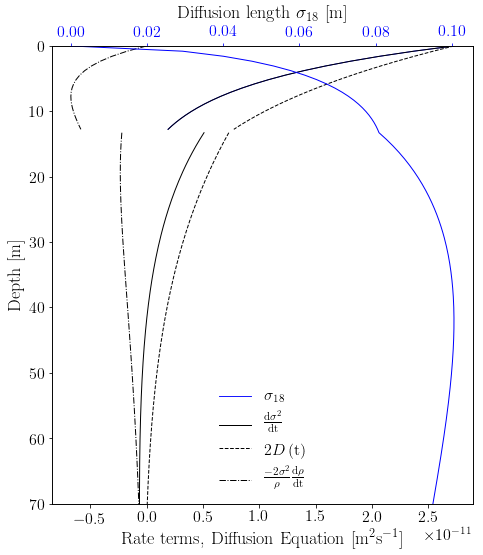
\includegraphics[width=0.6\textwidth]{Analytical_DiffLenEq_terms_SiteA.png}
		\caption{Contribution of the diffusion(dashed) and densification(dot-dashed) terms from Eq. \ref{Eq:dsigma2_dt} to the final analytical diffusion length solution (blue).}
		\label{Fig:ICE_DiffDensTerms}
	\end{figure}
	
	To simplify the work of this thesis, the numerical module of the CFM and the iso-CFM has not been implemented in the final computations, and the diffusion length profiles referred to in the rest of the project are calculated through an analytical method, using equations derived from Eq. \ref{Eq:dsigma2_dt} analytically. A short walk-through of the derivations will be presented here as they are described in \cite[Gkinis et al., 2021]{Gkinis2021}.
	By substitution of variables rearrangement Eq. \ref{Eq:dsigma2_dt} becomes:
	\begin{equation}
		\frac{\text{d}\sigma^2}{\text{d}\rho} + \frac{2\sigma^2}{\rho} = 2\left(\frac{\text{d}\rho}{\text{d}t}\right)^{-1}D(\rho)
		\label{Eq:dsigma_dt_rearrange}
	\end{equation}
	which can be converted to integral form:
	\begin{equation}
		\sigma^2(\rho) = \frac{1}{\rho^2}\int_{\rho_0}^{\rho}2\rho'^2\left(\frac{\text{d}\rho'}{\text{d}t}\right)^{-1}D(\rho')\text{d}\rho'
		\label{Eq:sigma2_rho_integral}
	\end{equation}
	Then, by using the densification rate parameterisation given in \cite[Herron and Langway, 1980]{HerronLangway1980}, the expression becomes:
	\begin{equation}
		\frac{\text{d}\rho(z)}{\text{d}t} = k(T)\, A^{\nu}\, (\rho_{\text{ice}} - \rho(z)),
		\label{Eq:drho_dt}
	\end{equation}
	where $k(T)$ is an Arrhenius-type densification rate constant, dependent on temperature and densification zone described by:
	\begin{equation}
		k_0(T) = 0.011\, \exp\left(-\frac{10160}{RT}\right), \qquad \nu_0 = 1
		\label{Eq:ArrCoeff_Zone1}
	\end{equation}
	in the upper densification zone, $\rho < 550 \rho_{\text{co}}$. In the lower densification zone, $\rho \geq \rho_{\text{co}}$, it is described as:
	\begin{equation}
		k_1(T) = 0.575\, \exp\left(-\frac{21400}{RT}\right), \qquad \nu_1 = 0.5.
		\label{Eq:ArrCoeff_Zone2}
	\end{equation}
	Using the parameterization of the diffusivity coefficient from Eq. \ref{Eq:DiffusivityConstant} and expressing the term $1/\tau = 1-b_{tau}\left(\frac{\rho}{\rho_{\text{ice}}}\right)^2$ in densities, the diffusivity coefficient can be described as a function of density:
	\begin{equation}
		D_i(\rho) = \frac{m \, p \, D_{\text{air}}}{R \, T \, \alpha_{s/v}^i}\left(1-b_{\tau}\left(\frac{\rho}{\rho_{\text{ice}}}\right)^2\right)\left(\frac{1}{\rho} - \frac{1}{\rho_{\text{ice}}}\right).
		\label{Eq:DiffusivityConstant_2}
	\end{equation}
	
	By then inserting in Eq. \ref{Eq:sigma2_rho_integral}, defining $\frac{m \, p \, D_{\text{air}}}{R \, T \, \alpha_{s/v}^i} = \zeta$, and integrating the final analytical equations for the diffusion length in upper and lower densification zones can be obtained:
	\begin{equation}
		\sigma^2(\rho < \rho_{\text{co}}) = \frac{\zeta}{\rho^2 \, k_0 \, A^{\nu_0} \rho_{\text{ice}}}	\left[\rho^2 - \rho_0 - \frac{b_{\tau}}{2\rho_{\text{ice}}^2}(\rho^4 - \rho_0^4)\right]
		\label{Eq:sigma2_Final_Zone1}
	\end{equation}
	
	\begin{equation}
		\begin{split}
			\sigma^2(\rho \geq \rho_{\text{co}}) = &\frac{\zeta}{\rho^2 \, k_1 \, A^{\nu_1} \rho_{\text{ice}}}	\left[\rho^2 - \rho_{\text{Cr}} - \frac{b_{\tau}}{2\rho_{\text{ice}}^2}(\rho^4 - \rho_{\text{Cr}}^4)\right] \\
			&+ \frac{\zeta}{\rho^2 \, k_0 \, A^{\nu_0} \rho_{\text{ice}}} \left[\rho_ {\text{Cr}}^2 - \rho_0 - \frac{b_{\tau}}{2\rho_{\text{ice}}^2}(\rho_{\text{Cr}}^4 - \rho_0^4)\right]
		\end{split}
		\label{Eq:sigma2_Final_Zone2}
	\end{equation}
	
	The analytical equations have been used for creating a contour plot of the analytical solutions for $\sigma_{18}$ at the close-off density, $\rho_{\text{co}}$. 
	
	\begin{figure}
		\centering
		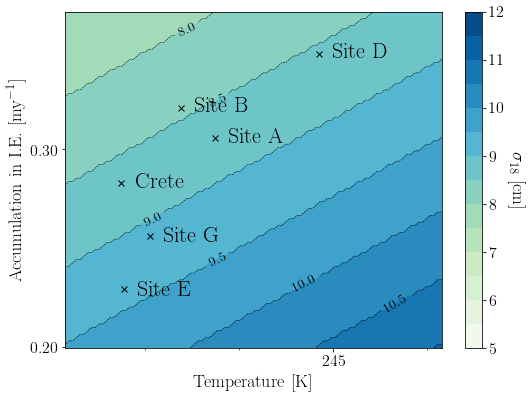
\includegraphics[width=0.7\textwidth]{ContourPlot_Alphabet.png}
		\caption{Crete and surrounding Alphabet cores, as their analytical solutions place them according to observed temperature and accumulation rate.}
		\label{Fig:ICE_ContourPlot}
	\end{figure}
	
	
	These analytical equations are used to compute diffusion lengths to compare with the optimal diffusion length estimates computed from the raw data. One could advantageously spend some time and energy on using the iso-CFM to numerically compute the comparison diffusion lengths with different temperature and accumulation forcing to recreate a diffusion length profile corresponding to the largest likelihood at a given drill site. Since the iso-CFM do consist of many different modules all with different possibilities for parameterisation, it is outside the scope of this project to develop a iso-CFM diffusion length estimate. In-depth methodology and results from the iso-CFM can be found in \cite[Gkinis et al., 2021]{Gkinis2021}.
	
	\begin{figure}
		\centering
		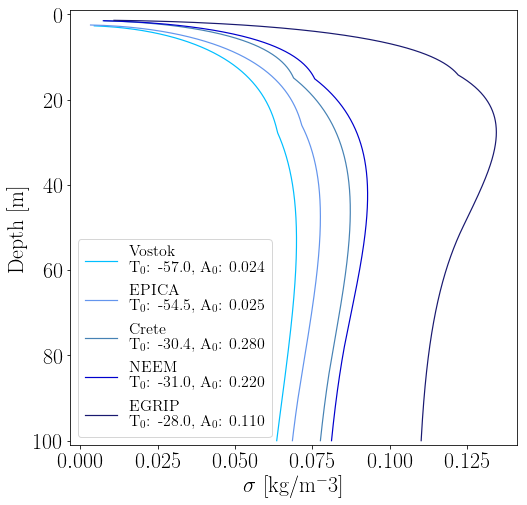
\includegraphics[width=0.7\textwidth]{DiffProf_Examples.png}
		\caption{Analytically calculated diffusion length profile examples given five different initial conditions representing present day conditions at the five different ice core locations. Temperature, $T_0$, is in $^{\text{o}}$C and accumulation, $A_0$, is in meter of water equivalent per year.}
		\label{Fig:DiffProf_Examples}
	\end{figure}
	
	
	\section[Temperature Estimation]{Temperature Estimation}
	\label{Sec:Ice_TempEstimation}
	Through the theoretically based analytical (or nummerical) estimates of the diffusion length, $\sigma_{\text{model}}$, and the diffusion length estimate from the isotopic signal of a depth section of an ice vore, $\sigma_{\text{firn}}$, a temperature estimate of can be given. This estimate made by numerically solving Eq. \ref{Eq:Firn_Temp_est_Roots} with $T$ as the unknown variable:
	\begin{equation}
		\left(\frac{\rho_{\text{co}}}{\rho_{\text{ice}}}\right)^2 \sigma_{\text{model}}^2(\rho=\rho_{\text{co}}, T(z), A(z)) = \sigma^2_{\text{firn}}
		\label{Eq:Firn_Temp_est_Roots2}
	\end{equation}. For the temperature estimates made in this project a secant numerical method\cite{Press2007} was used, through the Python \lstinline[language=Python]|SciPy| package \lstinline[language=Python]|scipy.optimize.newton|. Only the function it self is provided and no derivative is given, so the \lstinline[language=Python]|scipy.optimize.newton| uses the secant method to find a zero of the function passed. If a derivative was given, the packages would use a Newton-Raphson\cite{Press2007} scheme to find the zero of the function.
	
	
	
	\todo{ICE-TEMP.EST: Give an example of temperature estimation?}
	
	
	
	
	
	\section[ECM and DEP][ECM and DEP]{ECM and DEP}
	\label{Sec:Ice_ECMandDEP}
	Electrical conductivity measurements(ECM), dielectric profiling(DEP) and isotopic composition analysis are three distinct ways of analyzing an ice core to examine past temperatures, climate and atmospheric composition. Some of these methods are sensitive to violent volcanic eruptions, which makes it possible to use known eruptions visible in the ice cores as volcanic horizons, and thus making dating of the ice core more precise and absolute.
	\subsection[ECM][ECM]{Electrical Conductivity Measurements}
	\label{Sec:Ice_ECMandDEP_ECM}
	The conductivity of ice arises from the current emerging due to the build-up of space charges in the ice structure. This conductivity can be analyzed by measuring the electrical current(DC) - induced by the electric potential and the acid balance - between two electrodes which are moved along the ice cores length. This current will be connected to the acid impurity concentration (pH), in the form of $\text{H}_3\text{O}^+$ concentration, of the ice core. Higher levels of acid impurity concentration are due to volcanic eruptions. Large amounts of volcanic gases, i.e. $\text{SO}_2$, in the atmosphere oxidizes and combines with water to form acid, i.e. sulphuric acid, which is the washed out of the air due to precipitation. Thus it is made possible to recognize volcanic horizons in ice cores, and - if the location of the eruption is known - from the amount of acid, the magnitude of the eruption can also be estimated.\\
	High acidity of layers containing volcanic fall-out influence the dielectric constant of ice, so that these layers may be a possible explanation to the internal reflection horizons found in radio-echo sounding. \\
	The measured current can then be transformed into acidity by a calibration curve relating the current, in $\mu$A, to the acidity, in $\mu$equivalents $\text{H}_3\text{O}^+$ per kilogram. To find the calibration parameters, the current and the acidity must be measured - the current through the above mentioned method, and the acidity through pH measurements of melted ice core samples. The pH measurements must further be corrected for any $\text{co}_2$ induced $\text{H}^+$ ions (REFERENCES).The relation between acidity [$\text{H}^+$] (corrected for $\text{co}_2$ induced $\text{H}^+$) and current $I$ can be expressed in two ways:
	\begin{itemize}
		\item $[H^+] = (0.017\, I^2 + 1.2) \mu \text{equiv. H}^+ /\text{kg}$\\
		without a 50\% correction for $\text{co}_2$ surplus.
		\item $[H^+] = (0.045\, I^{1.73}) \mu \text{equiv. H}^+ /\text{kg}$\\
		with a 50\% correction for $\text{co}_2$ surplus.
	\end{itemize}
	The salt concentration in the ice can be estimated from measurements of the specific conductivity $\sigma$ of the melted samples. The salt contribution hereto can be expressed as:
	\begin{equation}
		\sigma_s = \sigma - \sigma(\text{H}^+) - \sigma(X^-) - \sigma(\text{HCO}_3^-)
	\end{equation}
	where the three later terms correspond to the contributions from $\text{H}^+$(through pH measurements) and its anions\footnotemark, $\text{HCO}_3^-$ and any other anions $X^-$. The anion concentration will be equal to the cation concentration, which in this case is only $\text{H}^+$ concentration. Disregarding low acidity samples, the concentration of $\text{HCO}_3^-$ is negligible and thus  $\text{concentration}(X^-) \approx \text{concentration}(\text{H}^+)$. 
	The current is thus heavily influenced on/determined by the $\text{H}^+$ concentration, and thus it is approximated that the salt concentration has no influence on the current readings, which is fortunate, since the ECM method only responds to acidity, and not to salt and ammonia concentrations. This is one of the methods limitations, which the later dielectric profiling method took into account.
	
	\footnotetext[2]{Anions are molecules losing a number of electrons to become negatively charged. Cations are molecules that gain a number of electrons to become positively charged.}
	\subsection[DEP][DEP]{Dielectric Profiling}
	\label{Sec:Ice_ECMandDEP_DEP}
	A method was later developed to demonstrate how both acids and salts play a decisive role in the determination of the electrical behavior of ice. The dielectric response of an ice core can be used to determine the total ionic concentration of the core. For ECM the measurements are sensitive to the fluctuating distance between ice core and electrodes, and after each measurement a fresh piece of ice needs to be prepared to repeat a measurement.\\
	A new dielectric profiling technique (DEP) was developed (REFERENCES) with the advantages over the ECM that no direct contact is needed between the electrodes and the ice, so that the ice can stay in a protective polythene sleeve and the experiment easily can be repeated on the same piece of ice. Together the ice core and the polythene sleeve creates a complete system, where the plastic acts as an electrical blocking layer.\\
	The dielectric response is measured by a sweeping of the AF-LF frequency range for the entire ice-polythene system. At LF the conductivity of the composite system is within a few percentages of the intrinsic behavior of the ice itself. At HF-VHF frequencies it also approximates well enough (REFERENCES).\\
	The measured dielectric parameters are the conductivity of ice at HF-VHF range, denoted $\sigma_{\infty}$ where $\infty$ signifies a frequency much higher than the relaxation frequency, $\text{f}_{\text{r}}$, of the dominant dispersion in the system. Both of these parameters display clear chemical response signals which can be used either alone or in combination with other ice core analysis measurements like ECM and isotope analysis.\\
	If the core under analysis is chemically analyzed for $\text{Na}^+$, $\text{Mg}^{2+}$, $\text{Cl}^-$, $\text{SO}_4^{2-}$ and $\text{NO}_3^-$, a number of important parameters, which can be used to evaluate the response of the dielectric parameters, can be calculated(REFERENCES):
	\begin{itemize}
		\item The salt parameter, which represents the total marine cation concentration calculated with the assumed marine ratios as:
		\begin{equation}
			[\text{salt}] = 1.05 ([\text{Na}^+] + [\text{Mg}^{2+}])
		\end{equation}
		\item $\text{XSO}_4$, the excess sulphate, which represents the amount the sulphate concentration is above the expected if the salt and sulphate ions were in normal sea salt ratios. Excess sulphate is essentially sulphuric acid, which is the main acidic component of the ice.
		\item The strong acid content of the ice has been calculated as(assuming no other ions present in significant quantities):
		\begin{equation}
			[\text{acid}] = [\text{Cl}^-] + [\text{SO}_4^{2-}] + [\text{NO}_3^-] - 1.05 ([\text{Na}^+] + [\text{Mg}^{2+}])
		\end{equation}
	\end{itemize}
	
	From data, it can be seen that acid and salt concentration peaks clearly affect $\sigma_{\infty}$ and $\text{f}_{\text{r}}$(EXAMPLES, REFERENCES). The relationship between salt and acid, and the two dielectric parameters have been derived through non-linear regression analysis. In PAPER(REFERENCES) the linear responses for the DEP at -22\degree C were:
	\begin{equation}
		\sigma_{\infty} = (0.39\pm 0.01)[\text{salt}] + (1.43\pm 0.05)[\text{acid}] + (12.7\pm 0.3)
	\end{equation}
	with 76.6 \% variance
	\begin{equation}
		\text{f}_{\text{r}} = (440\pm 11)[\text{salt}] + (612\pm 65)[\text{acid}] + (8200\pm 400)
	\end{equation}
	with 68.4 \% variance. $\sigma_{\infty}$ is measured in $\mu\text{S}/\text{m}$, $\text{f}_{\text{r}}$ in Hz and [acid] and [salt] in $\mu\text{Eq}/l$.
	The total ionic concentration of the ice core is strongly linked to the dielectric parameters, and a regression between the total anion concentration and the dielectric parameters gives:
	\begin{equation}
		[\text{anions}] = [\text{salt}] + [\text{acid}] = 0.022\sigma_{\infty}^{1.89} + 10^{-6}\text{f}_{\text{r}}^{1.61} - 0.2
	\end{equation}
	with 86.7 \% variance.
	
	The DEP complements the ECM technique by not only reacting to acids alone, as ECM does, but responds to both neutral salts and acids.
	The acid term is here associated with the DC conductivity, the same way it is also detected by ECM. The dielectric dependence on salts is consistent with the Bjerrum L defect\footnotemark affecting every one or two salt ions in the ice, indicating that a large fraction of the neutral salt is incorporated into the ice lattice.
	\footnote[3]{A Bjerrum defect is a crystallographic defect specific to ice, partly responsible for the electrical properties of ice. Usually a hydrogen bond will normally have one proton, but with a Bjerrum defect it will have either two protons (D defect) or no proton (L defect).(REFERENCES)}\\
	The sensitivity to salt concentrations allows for identifications of periods with major storms and open seas which are also important identifiers for paleo climate research, along with the volcanic eruption detection made possible through the ECM.
	
	
	
	\section[Volcanic Horizons][Volcanic Horizons]{Dating of Ice Cores Through Volcanic Horizons}
	\label{Sec:Ice_VolcanicHorizons}
	Throughout the history of the earth a number of different geophysicals events have left their mark on the geological and glaciological records we use to steal a glance into the past. When considering ice core records, there are few as visible - both to the eye and in measured data - than volcanic eruptions. It is widely known [REFERENCE] that eruptions above a certain scale have the possibility to change not only the atmospheric composition, due to the heavy amount of volcanic material slung into the air, but also the ability to impact the climate in the years following an enormous eruption. 
	Through electrical conductivity measurements it is possible to observe the very clear effects of some volcanic events in ice cores. Particles from the eruption are quickly transported from the source, since the atmospheric airflow will scatter the particles all over the atmosphere at a relatively high speed. Thus the dust(particle) and ECM signals pick up the volcanic signal faster than for example the isotopic signals. The isotopic signal reacts much slower, as it must be subjected to a change in global - and then following local - temperature, which might first show after a number of years. Thus ECM, DEP and dust measurements are good records to use for dating ice cores. Some eruptions are only great enough to show in ice cores located close to the volcanic source [REFERENCE], while others are of a magnitude impacting the entire globe, thus showing in almost all ice core records. These volcanic horizons are specifically good for synchronizing records, which is essential for developing knowledge about the geographically varying climate, temperatures and hemispherical dependency of the past. 
	For this thesis the volcanic horizons are especially important for developing
	
	
\end{document}